\chapter{Cahier des charges}

Dans cette partie nous allons détailler les différentes caractéristiques
de notre projet. Nous allons commencer par étudier les différents objectifs
du projet puis nous l’analyserons plus en détail aux moyens d’outils de spécification.

\section{Les objectifs}

Les différents objectifs sont illustrés par le schéma en fin de section. Celui-ci,
bien que complexe, peut aider le lecteur à comprendre les liens entre tous les objectifs.
Les éléments \textbf{en gras} nous sont fournis et sont à intégrer dans le projet.

\paragraph{}
\begin{mdframed}[frametitle={Schéma représentant les différents objectifs du projet}, innerbottommargin=10]
\begin{center}
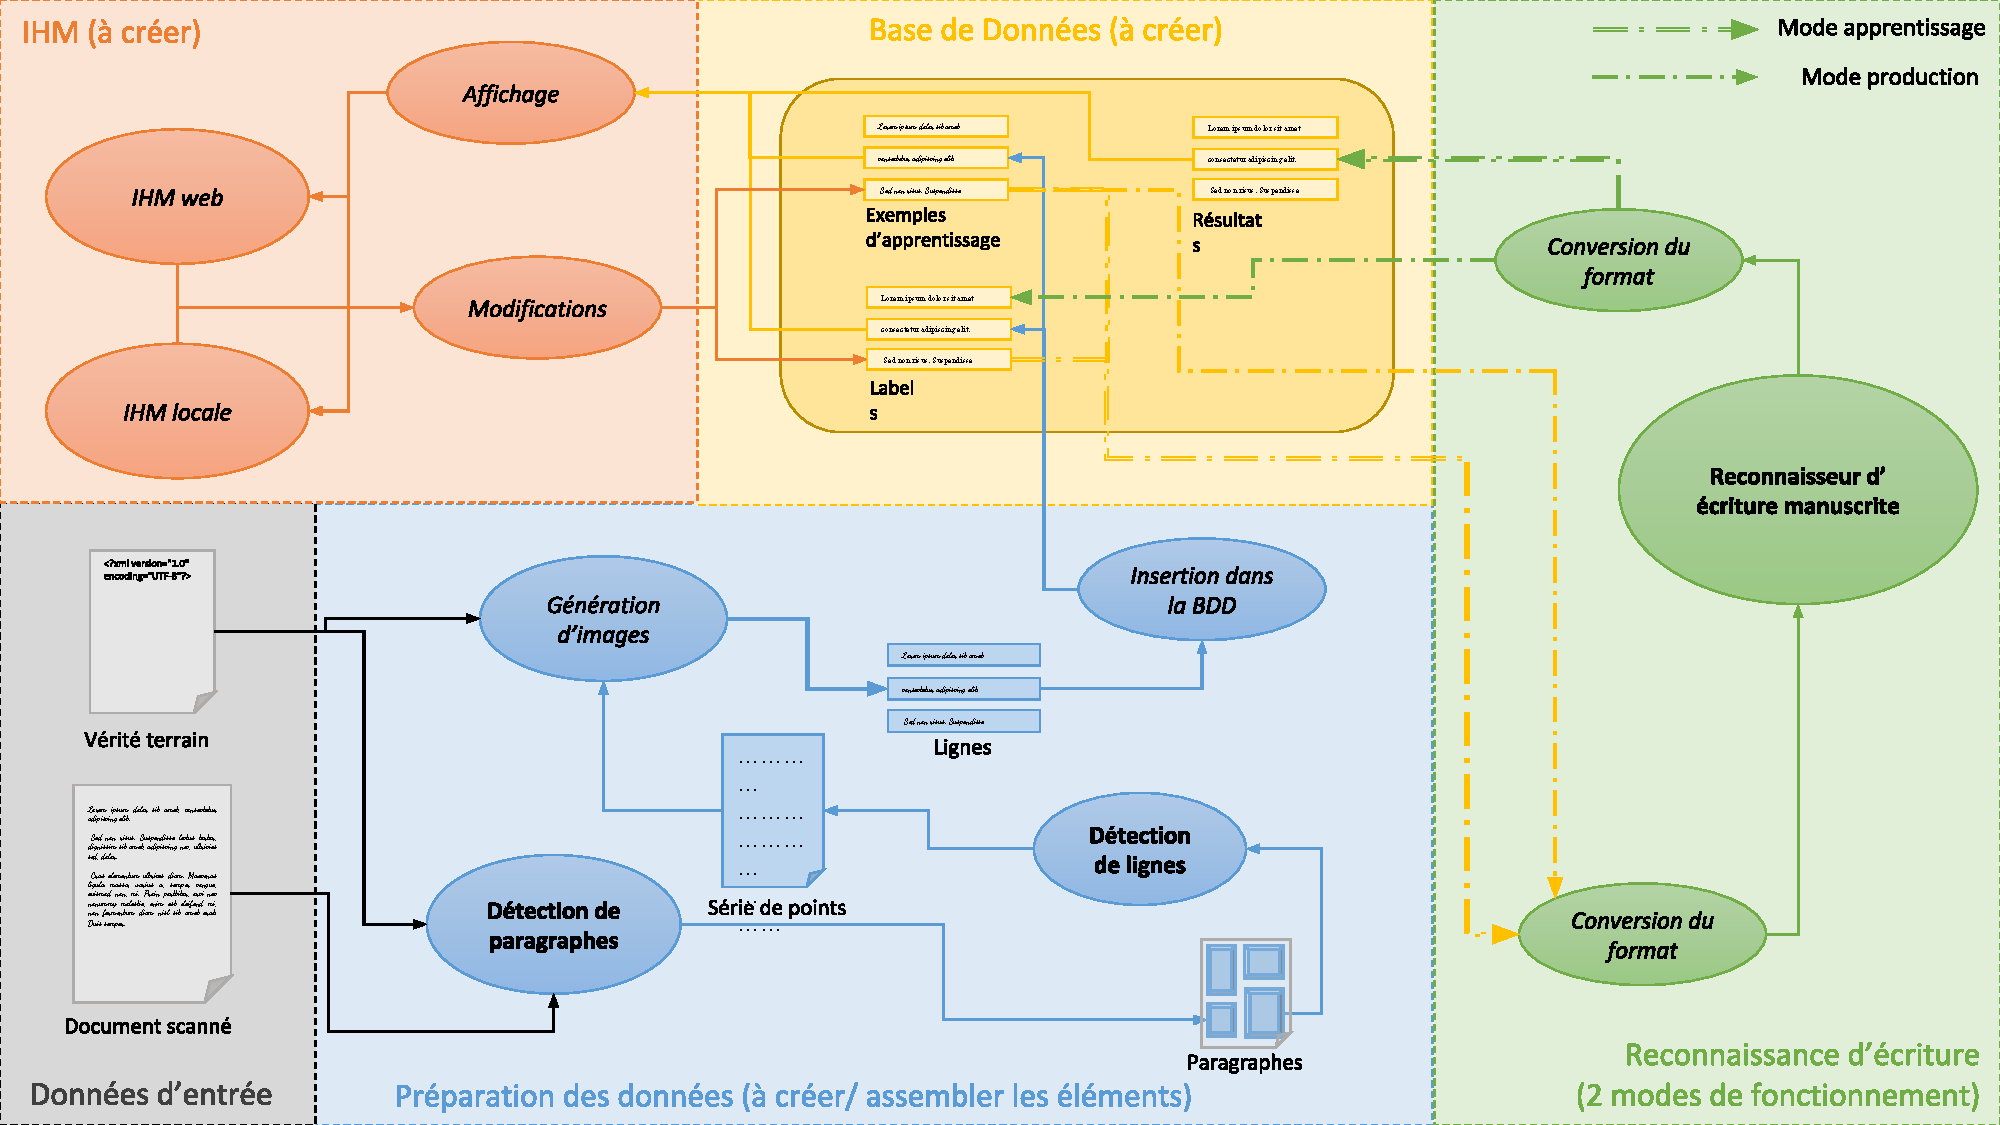
\includegraphics[width=\linewidth]{schema.pdf}
\end{center}
\end{mdframed}

\paragraph{}
Le premier objectif est de découper correctement les documents manuscrits sous la forme
d’imagettes. Ces imagettes peuvent correspondre à des lignes ou à des paragraphes des documents initiaux.
Le schéma ci-dessus représente un mode de fonctionnement dans lequel chaque imagette contient
une seule ligne du document, mais le projet doit contenir un second mode dans lequel chaque imagette
représente un paragraphe et où la fonction de détection de ligne est absente.

\paragraph{}
Le découpage en lignes se fait à l’aide d’un \textbf{outil de détection de lignes} et d’un
\textbf{outil de découpage de paragraphes}. Cette partie correspond à la zone du schéma sur fond bleu.
Le projet doit donc permettre de générer des imagettes en se passant du premier outil mentionné.

\paragraph{}
Dans la première version, le \textit{scan} d’un document contenant des informations manuscrites est
donné en entrée et est découpé en paragraphes grâce aux \textbf{données de position} présentes dans
les fichiers de la \textbf{base Maurdor} (contenant les scans des documents et leur vérité terrain).
Ces paragraphes sont par la suite découpés en lignes via l’outil détecteur de lignes. Les éléments obtenus
sont enfin convertis en imagettes avec un programme à créer appelé \textit{Génération d’images} sur le schéma.

\paragraph{}
Le deuxième objectif est de relier les imagettes à leur retranscription numérique
(aussi appelée vérité terrain). Cet objectif est réalisable grâce aux données de position
qui accompagnent les retranscriptions de la base Maurdor. Ces couples \texttt{(imagette, retranscription)}
seront ensuite enregistrés dans une base de données qui constituera la base d’apprentissage du
\textbf{système de reconnaissance d’écriture manuscrite}. Cette partie correspond également à la partie
en bleu du schéma. Une vérité terrain permet non seulement d’identifier les paragraphes mais
également de lier les imagettes à la retranscription numérique du texte manuscrit qu’elles contiennent
grâce aux informations de numéro de ligne. Il est possible que la vérité terrain ne soit pas toujours
fournie en entrée, le logiciel doit alors permettre à l’utilisateur de rentrer lui-même une retranscription
numérique (mode ajout utilisateur sur le schéma). Les imagettes (ou lignes sur le schéma) sont stockées
dans la base de données, en jaune. La base de données contient donc des imagettes (\textit{Exemples d’apprentissage}),
pouvant être associées à leur retranscription numérique (\textit{Label}) et à un texte généré par un
reconnaisseur d’écriture manuscrite (\textit{Résultats}).

\paragraph{}
Le troisième objectif est de générer les couples \texttt{(imagette, retranscription)} avec un format spécifique
qui pourra ensuite être facilement modifié, cela dans le but d’être compatible avec les formats d’entrée de
plusieurs systèmes de reconnaissance d’écriture manuscrite sans trop d’efforts.
Plusieurs choix s’offrent à nous. Comme les données en entrée sont dans le
\href{https://lampsrv02.umiacs.umd.edu/projdb/project.php?id=53}{format GEDI}, nous pourrions générer des
fichiers dans ce même format. Nous pouvons également les sauvegarder au format PiFF\cite{piff:2017},
fortement compatible avec ce type de données. Dans tous les cas, nous devrons créer un script qui
convertira les données (GEDI ou PiFF) en un format compatible avec le logiciel de reconnaissance d’écriture
manuscrite en notre possession. Le passage par le format GEDI ou PiFF permettra simplement de rendre les données
plus manipulables pour des personnes souhaitant les exploiter. Le système de reconnaissance d’écriture manuscrite
est situé dans la partie verte du schéma. Le logiciel devra permettre de générer trois jeux de données différents
associés à trois modes de fonctionnement du reconnaisseur :

\begin{itemize}
\item un mode d’\textbf{apprentissage} : dans ce mode, le système de reconnaissance extrait de la base de données les
imagettes et leur label associé pour pouvoir s'entraîner; il fournit ensuite un résultat pour chaque imagette,
qui pourra être comparé par des utilisateurs via une IHM;
\item un mode d’\textbf{évaluation} : ce mode permet de vérifier la qualité du reconnaisseur après un apprentissage;
\item un mode de \textbf{production} : dans ce mode, le reconnaisseur est censé être bien entraîné; il n’a que les
imagettes en entrée et il fournit une retranscription numérique (un label) pour des documents sans vérité terrain.
Il permet alors d’aider l’utilisateur à retranscrire numériquement un document manuscrit scanné.
\end{itemize}

\paragraph{}
Ces modes sont illustrés dans les schémas ci-dessous. Le premier schéma représente le mode évaluation avec l’option
de détection des lignes, et le second schéma représente le mode production sans cette option. Ceci est fait dans un
but illustratif, car les deux modes devront pouvoir être exécutés avec et sans cette option.

\newpage

\paragraph{}
\begin{mdframed}[frametitle={Schéma résumant le mode évaluation du projet (avec détection de lignes)}, innerbottommargin=10]
\begin{center}
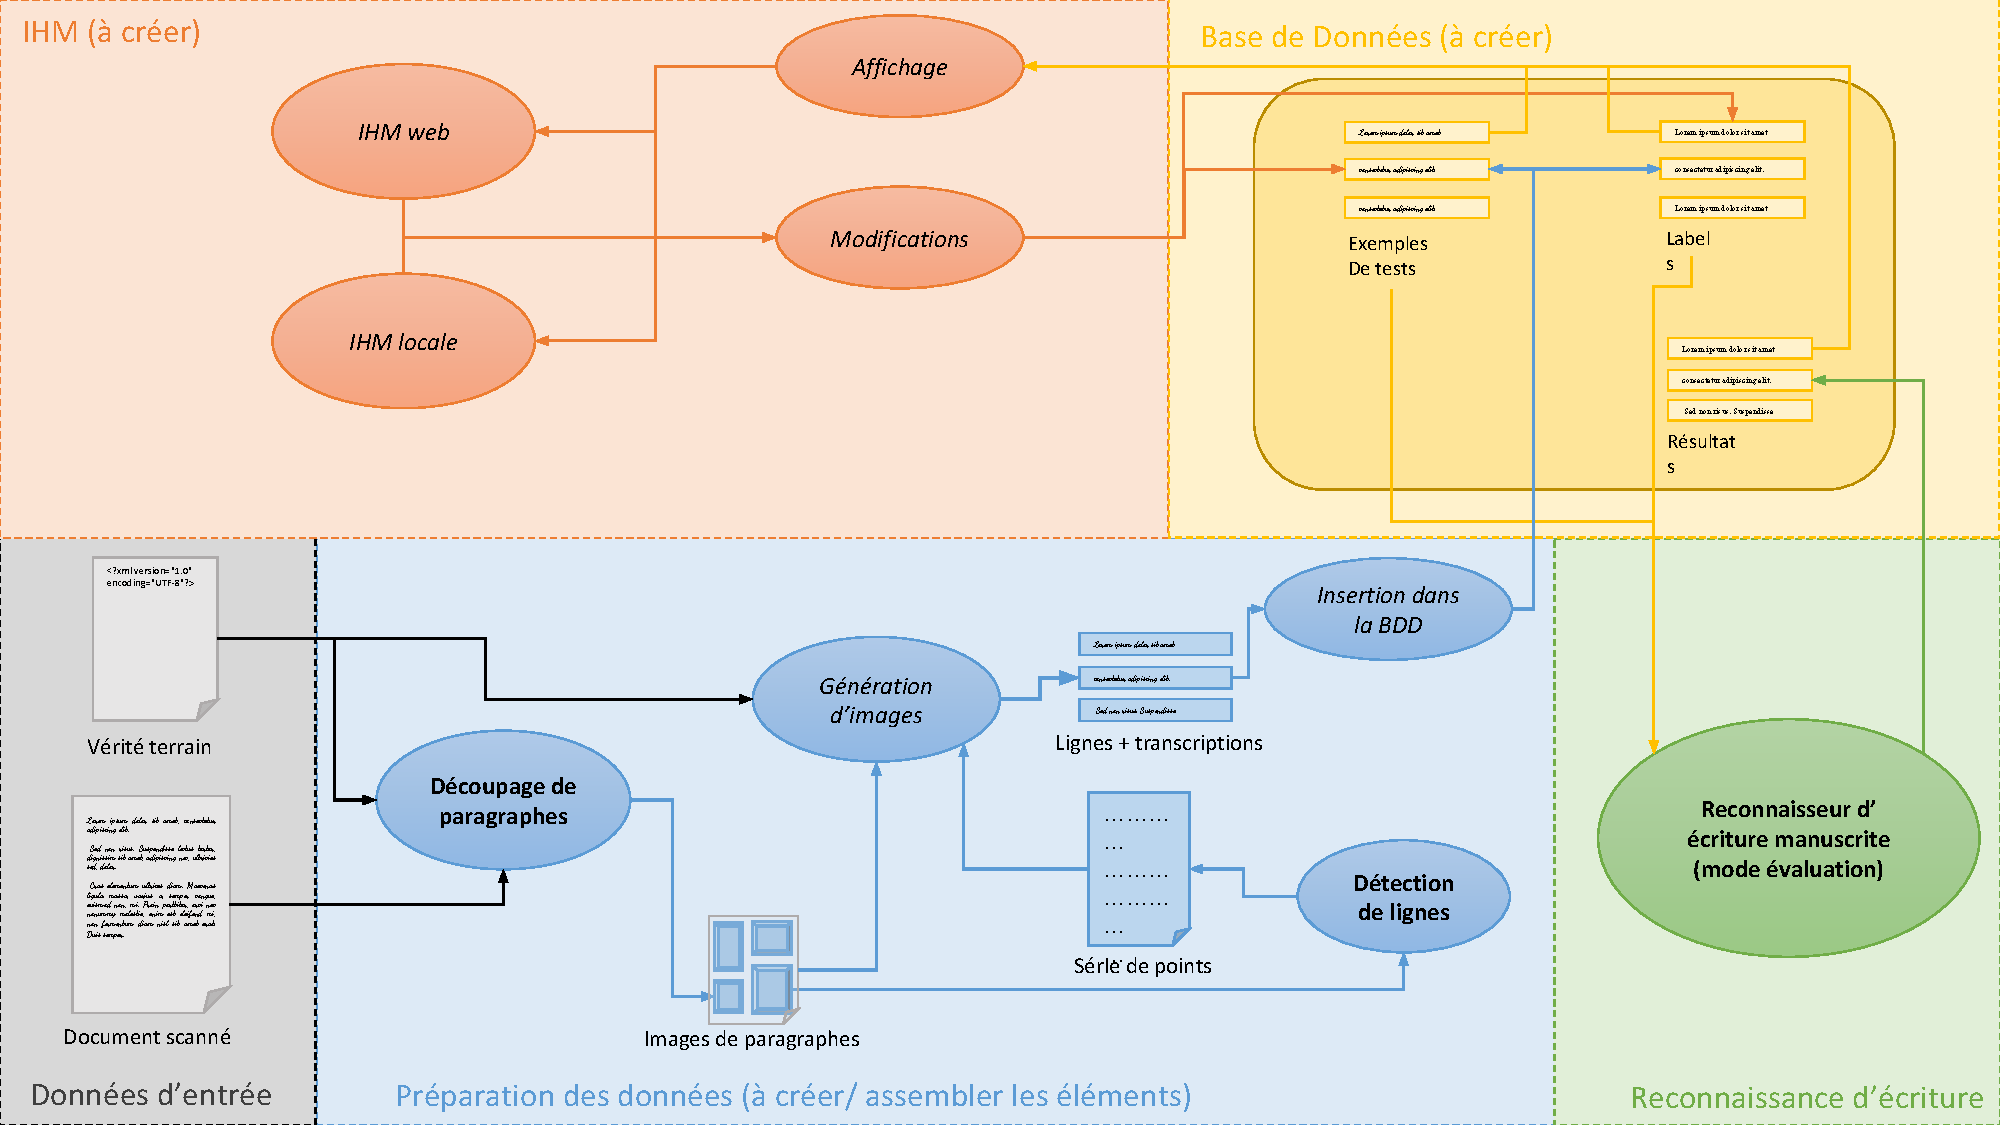
\includegraphics[width=\linewidth]{schema-eval.pdf}
\end{center}
\end{mdframed}

\paragraph{}
\begin{mdframed}[frametitle={Schéma résumant le mode production du projet (sans détection de lignes)}, innerbottommargin=10]
\begin{center}
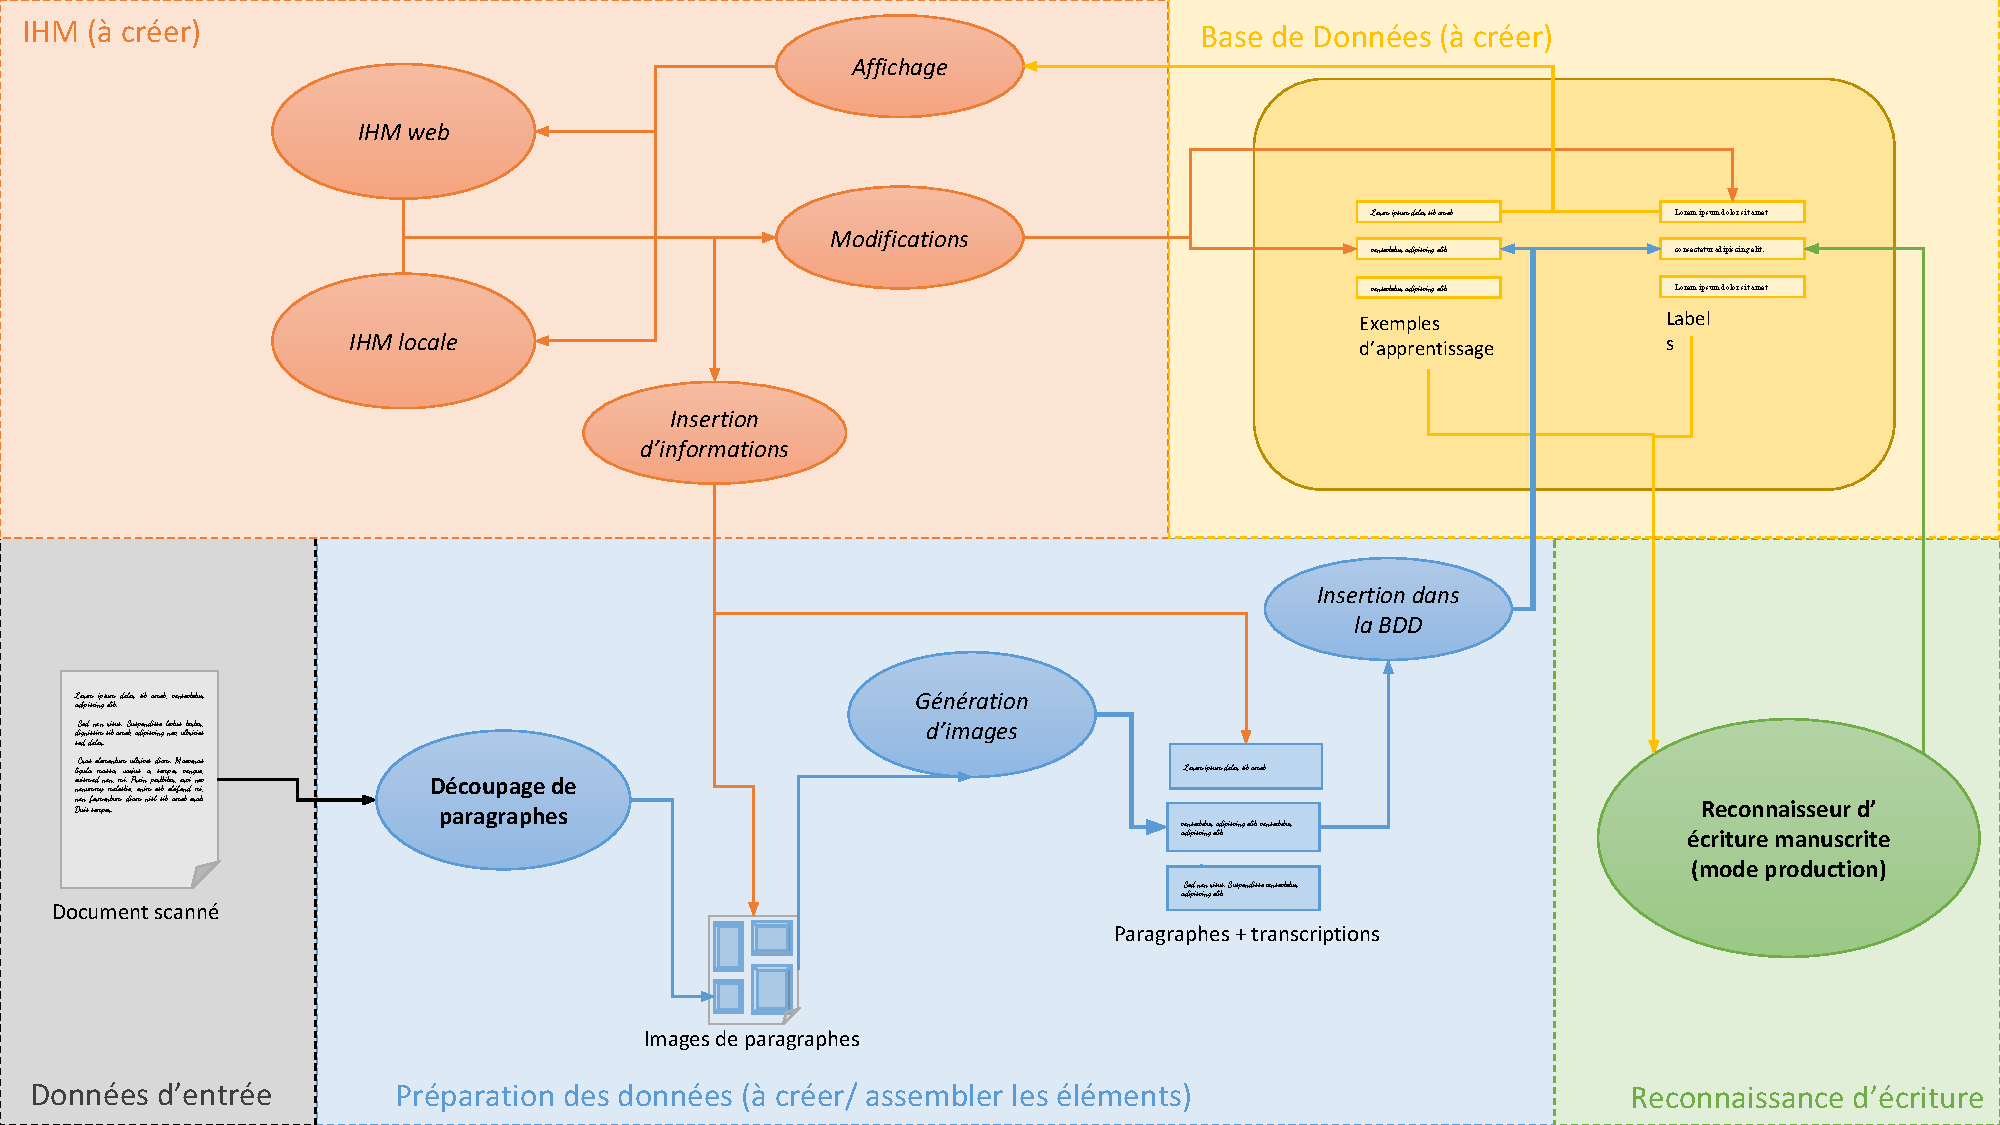
\includegraphics[width=\linewidth]{schema-prod.pdf}
\end{center}
\end{mdframed}

\newpage
\paragraph{}
Le quatrième objectif est de créer une Interface Homme-Machine (IHM) permettant d’observer les imagettes
et les retranscriptions, afin de confirmer et/ou corriger les retranscriptions si jamais elles ne correspondent
pas au texte de l’imagette. On doit également pouvoir supprimer des couples \texttt{(imagette, retranscription)}
de la base de données si jamais l’utilisateur considère qu’elles n’apporteront rien de bénéfique
à l’apprentissage du reconnaisseur. Les données que l'on pourrait vouloir supprimer seraient des
données trop bruitées, trop dégradées, mal coupées, etc. Il pourrait cependant être intéressant
de les conserver pour que le reconnaisseur apprenne à reconnaître des textes abîmés. Cet objectif est représenté
dans la partie rouge du schéma, l'IHM locale, qui doit pouvoir accéder à la base de données et la modifier.

\paragraph{}
Enfin, le dernier objectif (optionnel) est de créer une seconde interface permettant
d’observer les imagettes et les résultats du reconnaisseur. Cet objectif est optionnel
car il sort légèrement du cadre du travail qui nous est demandé mais il sera utile pour faire
une démonstration du reconnaisseur lors de la présentation finale de notre projet.
Nous pourrons ainsi montrer ce que notre travail aura pu apporter à la reconnaissance
d’écriture manuscrite. Cette tâche ne sera probablement pas longue à réaliser car elle peut
consister en une amélioration de l’IHM précédente. Pour rendre la démonstration plus
ludique, on pourrait aussi imaginer créer une IHM sous forme de jeu entre une personne
et le reconnaisseur. Par exemple, la personne et le reconnaisseur pourraient avoir à
retranscrire un texte manuscrit le plus vite possible. Cet objectif est représenté dans
la partie rouge du schéma, l'IHM web, qui doit comme la première interface
accéder à la base de données et la modifier.

\section{Description fonctionnelle des besoins}

\subsection{Diagramme bête à cornes}

Le diagramme suivant permet d’exprimer le besoin lié au projet. Ainsi, notre logiciel de
traitement de données manuscrites aura pour but principal de préparer et stocker des données
d’apprentissage pour le système de reconnaissance d’écriture manuscrite développé par Doptim.

\paragraph{}
\begin{mdframed}
\begin{center}
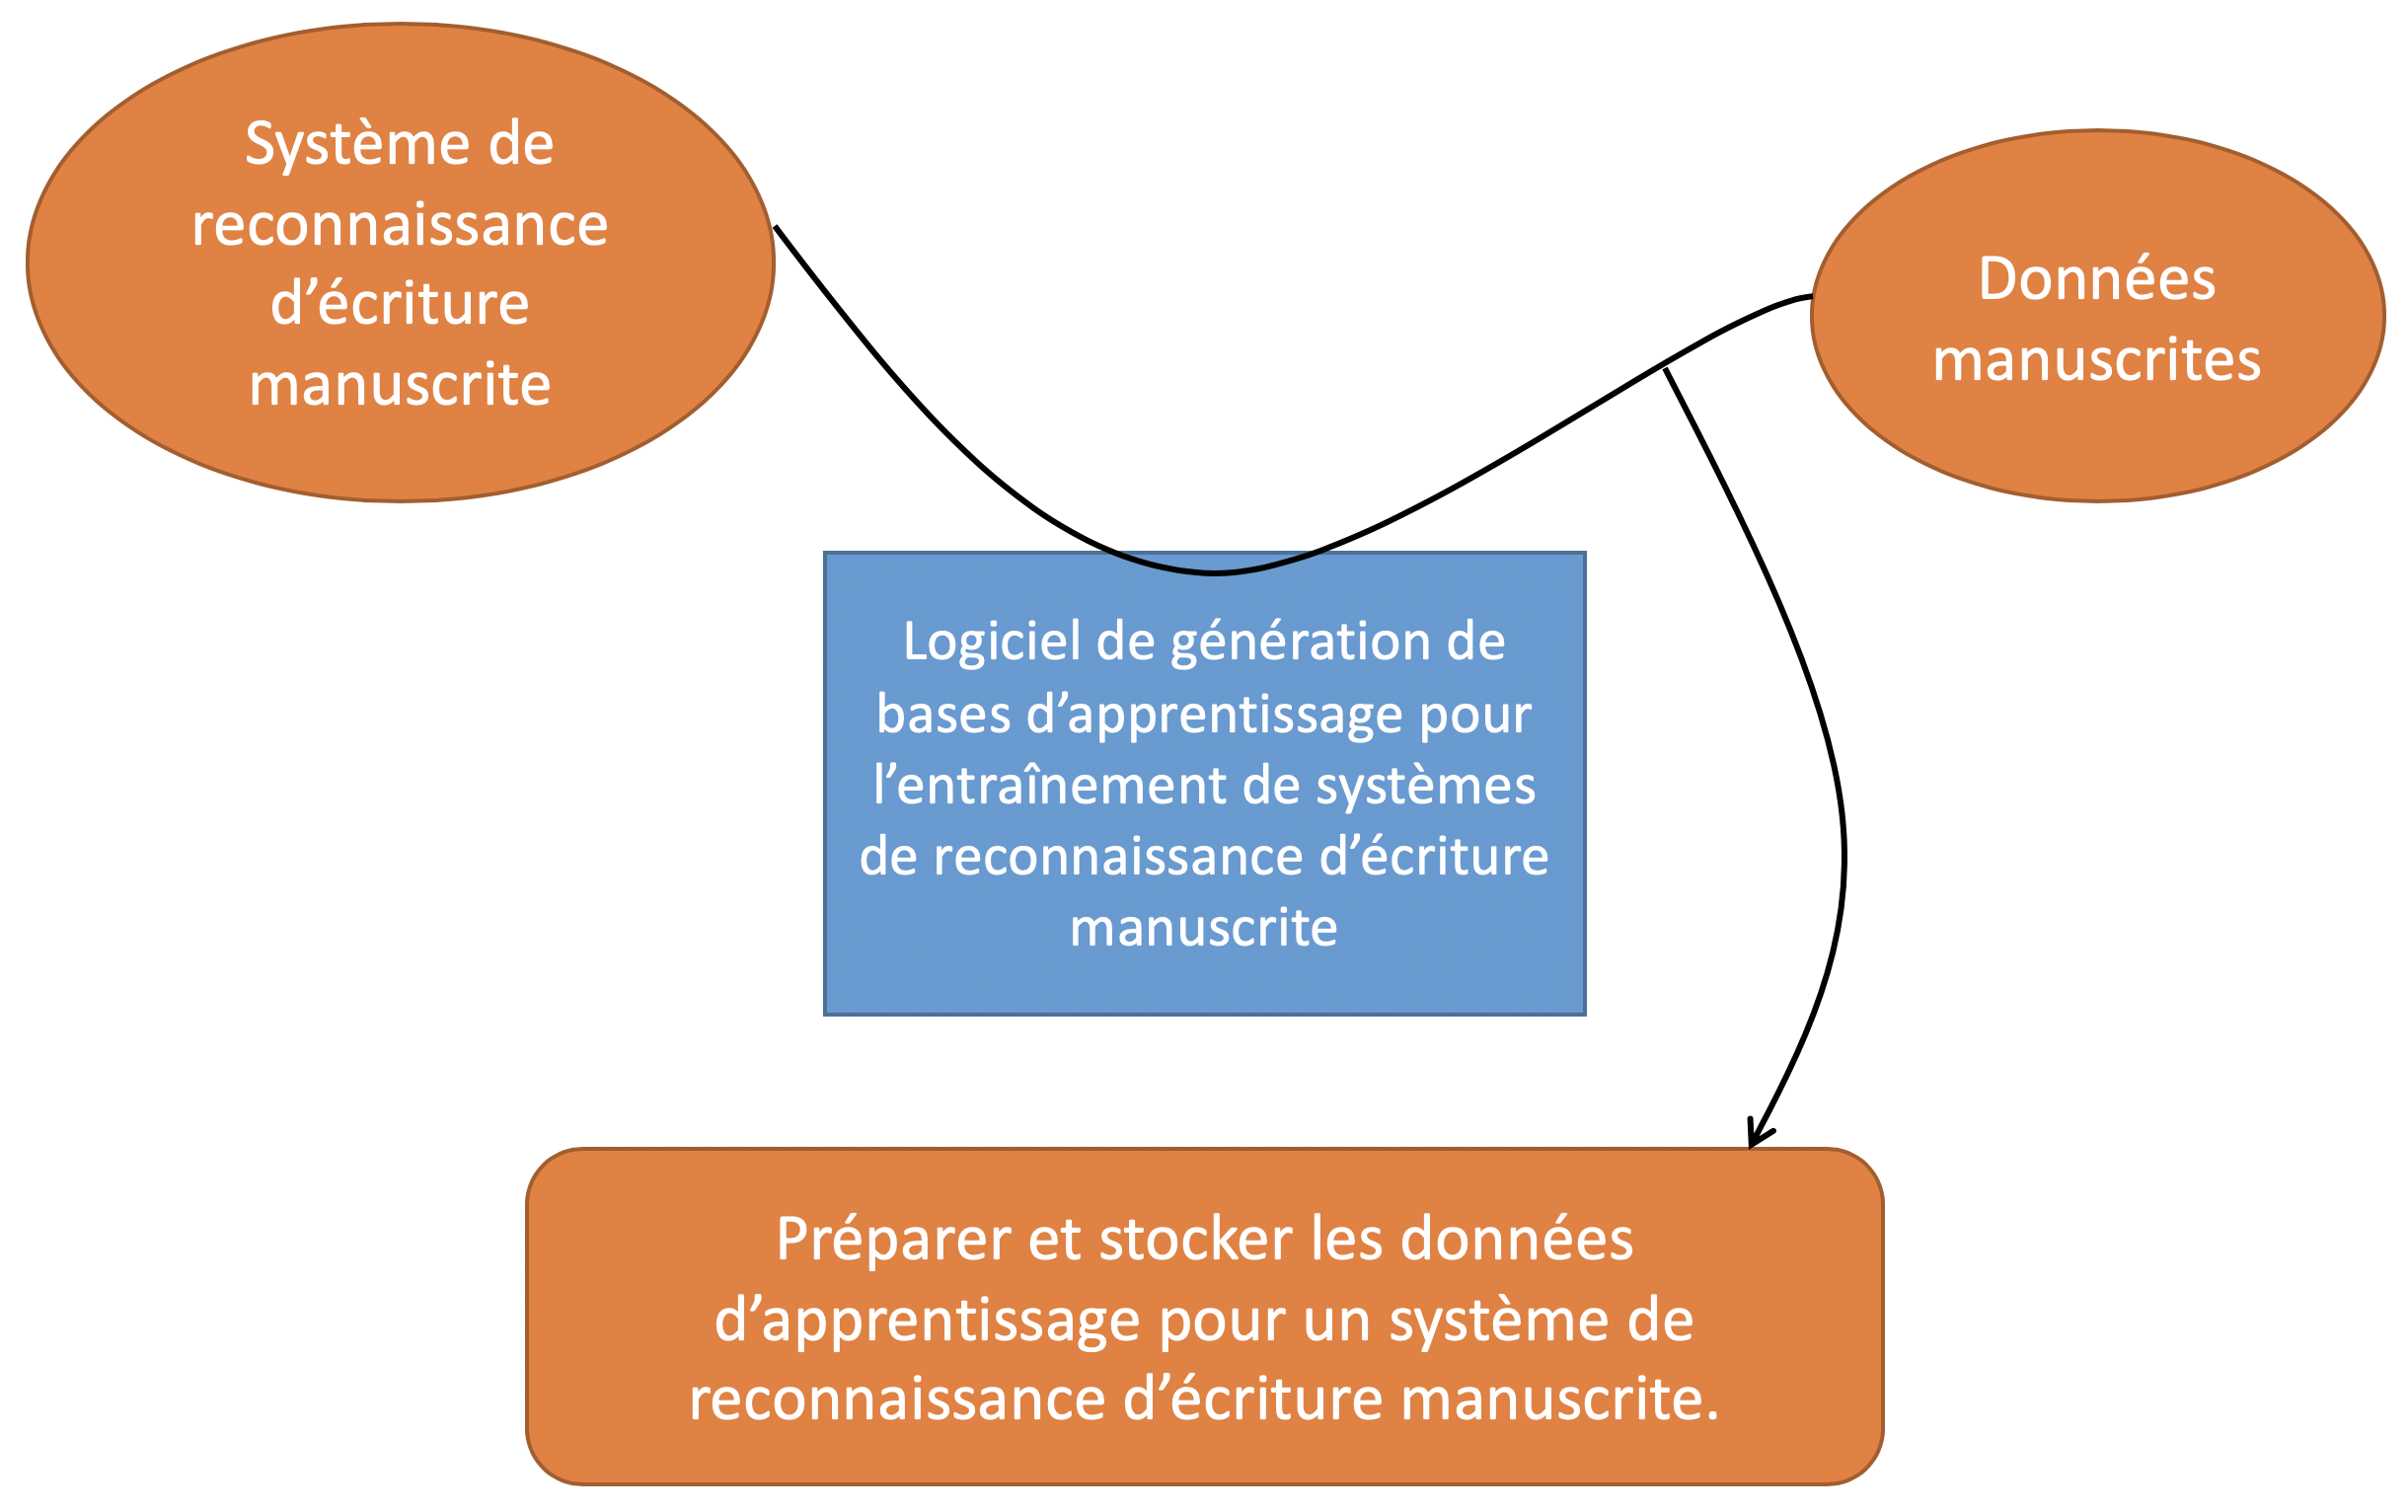
\includegraphics[width=0.7\linewidth]{bete-a-cornes.png}
\end{center}
\end{mdframed}

\newpage
\subsection{Diagramme pieuvre}

Le diagramme pieuvre, quant à lui, permet d’exprimer les différentes fonctions contraintes
qui découlent de l’objectif principal du projet. De ce fait, notre logiciel devra interagir
avec différents acteurs afin de s’intégrer parfaitement dans l’optique du projet :

\begin{itemize}
\item \textbf{FP1} : Tout d’abord, le premier objectif (et l’objectif principal du projet) est
de préparer et stocker les données d’apprentissage pour un système de reconnaissance d’écriture manuscrite.
\item \textbf{FC1} : Ensuite, il devra utiliser le détecteur de lignes fourni afin de découper
les phrases des textes d’entrée en imagettes. 
\item \textbf{FC2} : Il devra également permettre à l’utilisateur d’interagir avec les données
traitées afin de les vérifier et/ou de les modifier si nécessaire, le tout par le biais d’une Interface Homme-Machine. 
\item \textbf{FC3} : Notre logiciel utilisera aussi la vérité terrain fournie afin d’associer
les imagettes découpées à la bonne transcription.
\item \textbf{FC4} : Il faudra également que celui-ci soit compatible avec le format des données
qui lui seront fournies en entrée (format GEDI ou PiFF).
\item \textbf{FC5} : Enfin, notre logiciel devra regrouper les données afin de les stocker dans une base de données.
\end{itemize}

\paragraph{}
\begin{mdframed}
\begin{center}
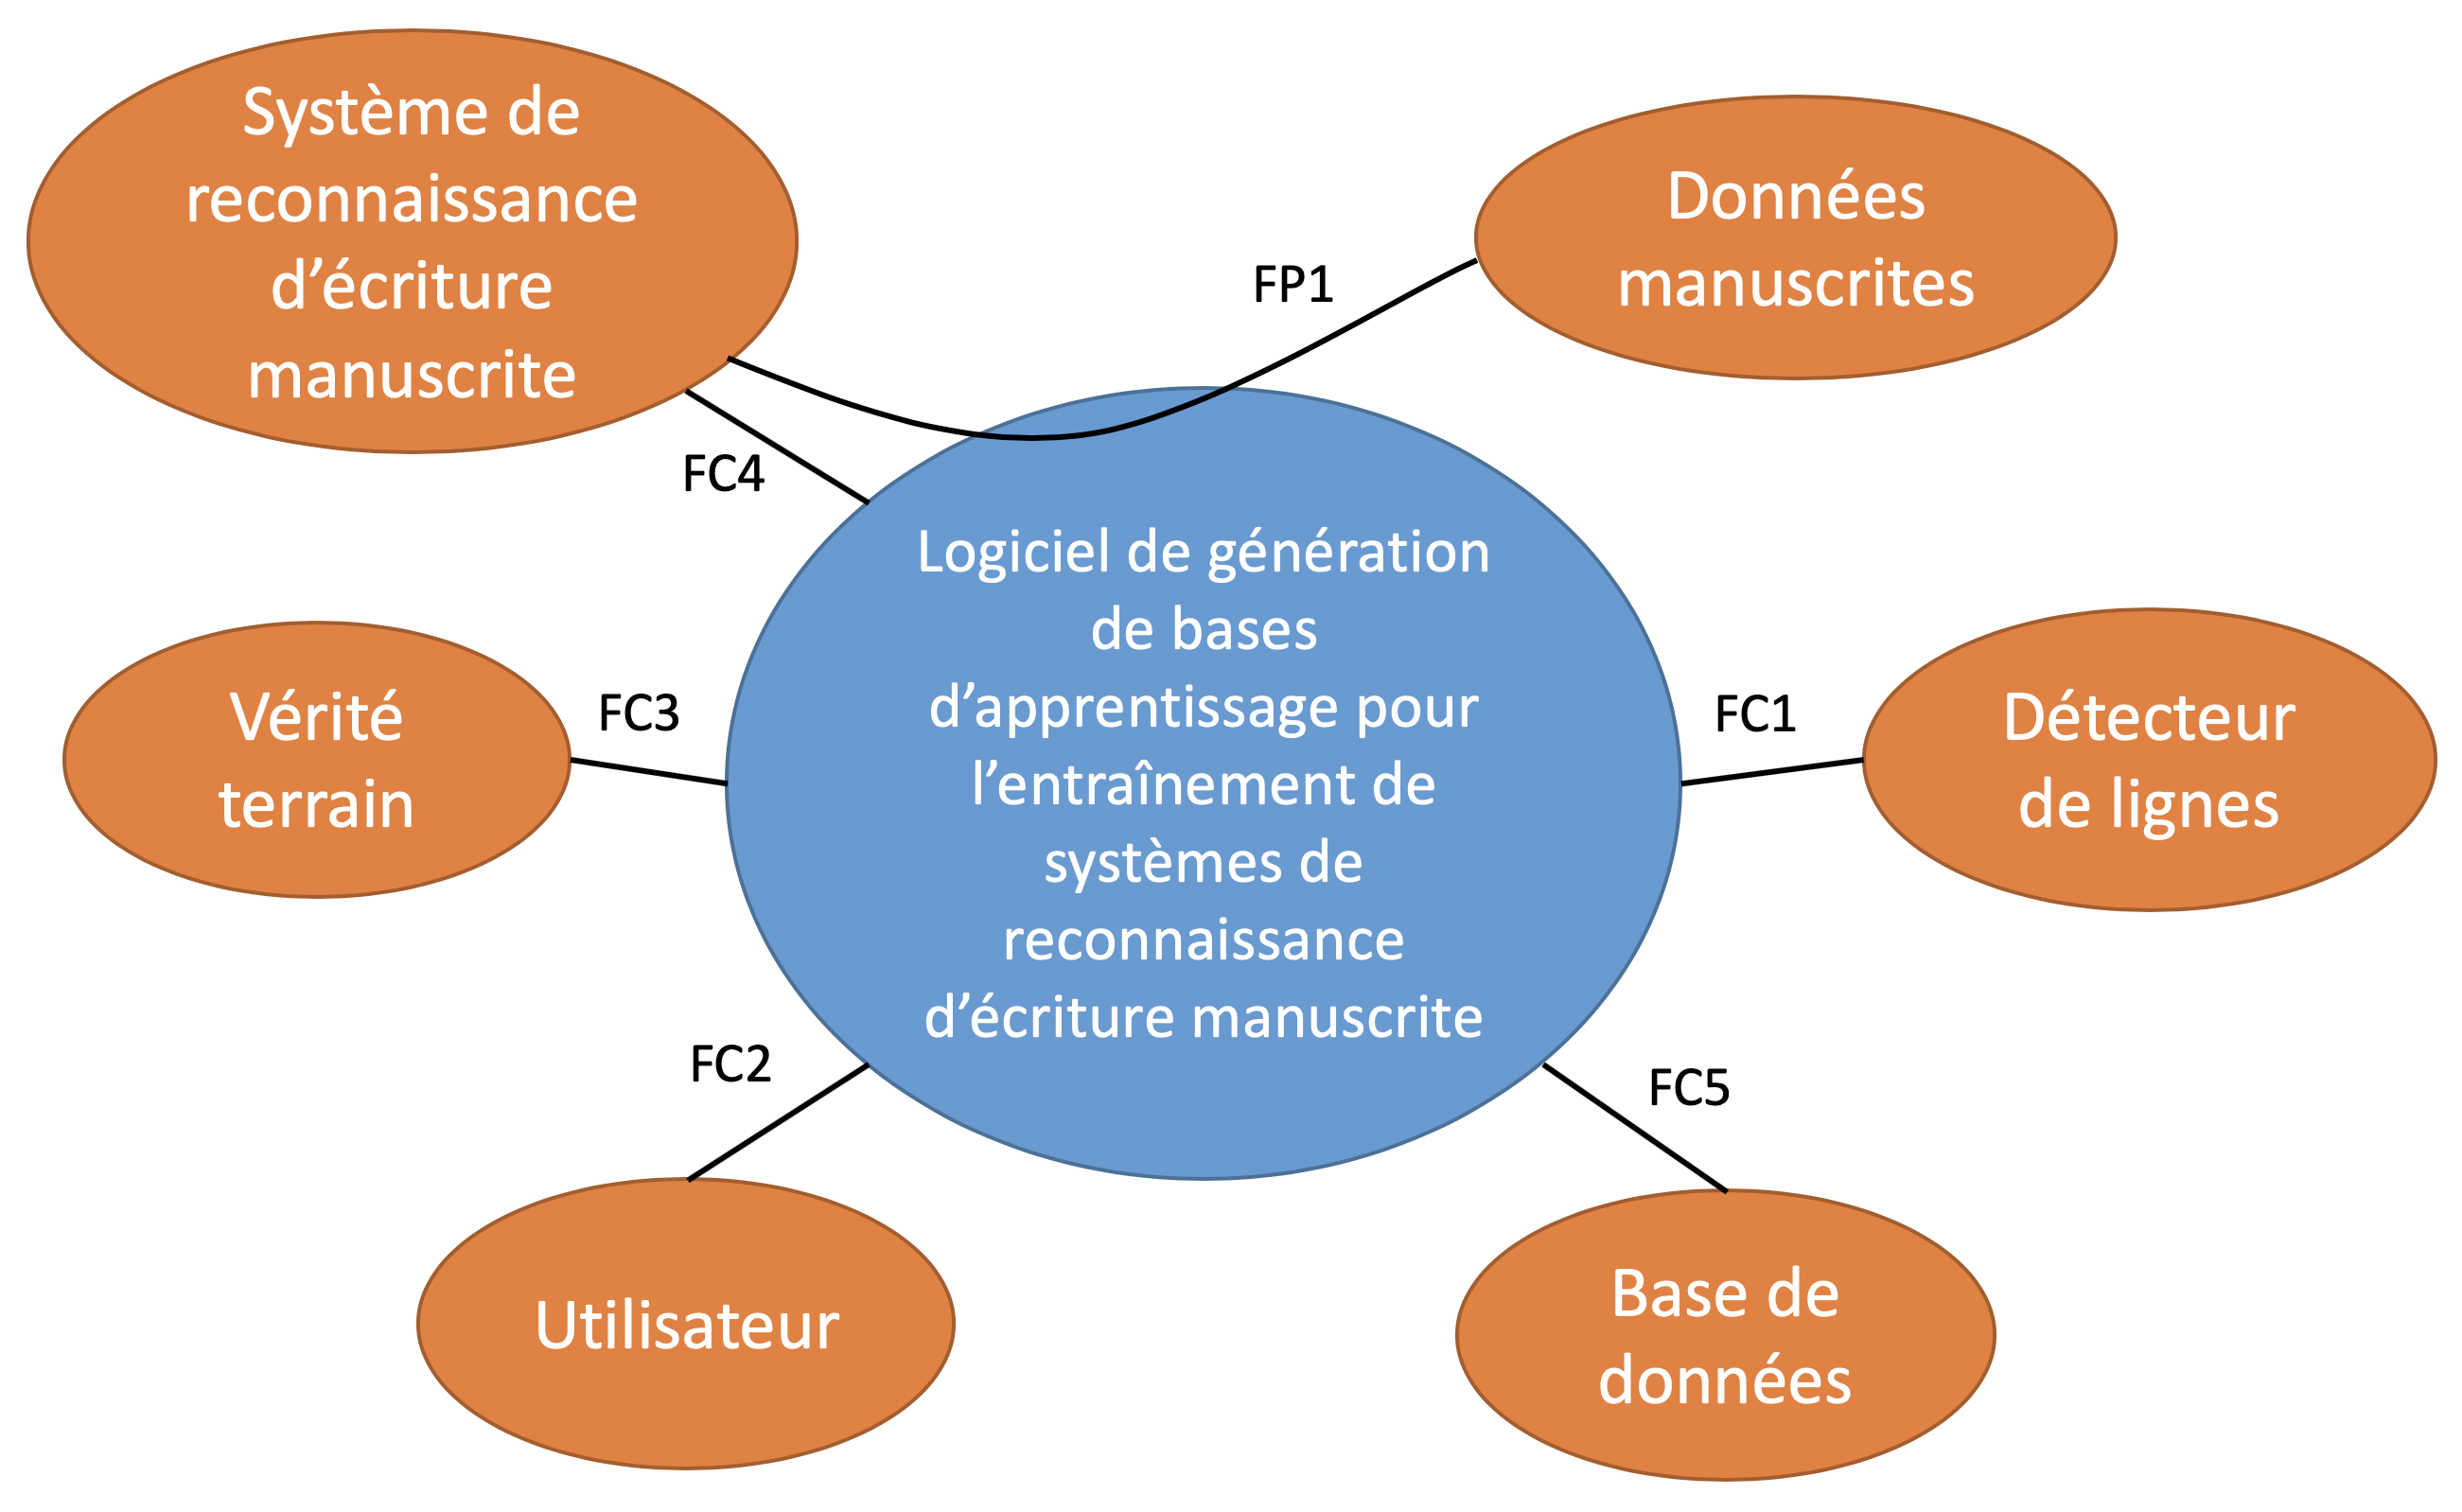
\includegraphics[width=0.7\linewidth]{pieuvre.png}
\end{center}
\end{mdframed}